\documentclass[12pt,oneside,a4paper]{article}

\usepackage{./custom}
\usepackage{array,multirow,makecell}
\usepackage{colortbl}
\usepackage{booktabs}
\usepackage{longtable}


\begin{document}
% title (fold)\begin{center}
\begin{titlepage}
\begin{center}

% Upper part of the page. The '~' is needed because \\
% only works if a paragraph has started.


\includegraphics[scale=0.5]{./img/dauphine_logo} \\[1.5cm]

% \textsc{\LARGE \textsc{CentraleSupélec}}\\[1.5cm]


\vfill
% Title
\rule{\textwidth}{1.6pt}\vspace*{-\baselineskip}\vspace*{2pt} % Thick horizontal line
\rule{\textwidth}{0.4pt}\\[\baselineskip] % Thin horizontal line
{ \huge  \textsc{Synthèse} \\[0.4cm]
\textsc{Microéconomie} }
\rule{\textwidth}{0.4pt}\vspace*{-\baselineskip}\vspace{3.2pt} % Thin horizontal line
\rule{\textwidth}{1.6pt}\\[1.5cm] % Thick horizontal line

\vfill
\paragraph{Foreword}
Any error or contribution should be reported
in the form of an issue, or a pull request for those
who can use \texttt{git} and \LaTeX, to
\begin{center}
  \url{https://github.com/mbataillou/Summaries/tree/master/Dauphine/Micro}
\end{center}
You can notice that there is always place for improvement
and your help is therefore welcome.
\vspace{\baselineskip}

\vfill
% Author
{\large
\begin{center}
  % \adfast{1}  \hspace{0.5cm}\textsc{\textbf{Encadrant du projet}}\hspace{0.5cm}   \adfast{1}  \\[0.3cm] \large
  {\Large  \hspace{0.5cm} \textbf{Auteurs} \hspace{0.5cm}   } \\[0.3cm]
  % \adfast{1}  \hspace{0.5cm}\textsc{Nom des élèves} \hspace{0.5cm}   \adfast{1} \\[0.3cm] \large
	\textsc{Bataillou Almagro} Marc \\
	  ---
\end{center}
}
\vfill

% Bottom of the page
{\large \today}

\end{center}
\end{titlepage}
% title (end)
 
 \newpage
{\hypersetup{linkcolor=black} \tableofcontents}


\newpage


\section{L'analyse financière} % (fold)
\label{sec:l_analyse_financiere}


\subsection{Introduction} % (fold)
\label{sub:introduction}

Il est important d'introduire les 3 principes fondamentaux de l'analyse financière :

\begin{itemize}[label=\ding{69}]

	\item Tout ce que j'ai, je le dois.

	\item Rien ne se perd, rien ne se crée, tous se transforme.

	\item Emplois durables financés pas des ressources durables

\end{itemize}

% subsection introduction (end)

\subsection{Les soldes intermediares de gestion} % (fold)
\label{sub:les_soldes_intermediares_de_gestion}

Il s'agit d'un reclassement du compte de résultat pour réaliser l'analyse financière.

\vfill

	\begin{center}
		\begin{tabular}{|c|}
		\hline
		\rule[-0.4cm]{0mm}{1cm}\textsc{Résultat d'EXPLOITATION}\tabularnewline
		\hline
		\rule[-0.4cm]{0mm}{1cm}\textsc{Résultat FINANCIER}\tabularnewline
		\hline
		\rule[-0.4cm]{0mm}{1cm}\textbf{\textsc{Résultat courant avant impôts}}\tabularnewline
		\hline
		\rule[-0.4cm]{0mm}{1cm}\textsc{Résultat EXCEPTIONNEL}\tabularnewline
		\hline	
		\rule[-0.4cm]{0mm}{1cm}\textbf{\textsc{Résultat net}}\tabularnewline
		\hline
		\end{tabular}
			\captionof{table}{Le compte de résultat}
	\end{center}
\vfill
	\begin{tabular}{|c|c|}
	\hline
	 \rule[-0.4cm]{0mm}{1cm}\textsc{\textbf{Marge comerciale}} &\multirow{2}*{\textsc{\textbf{Marge brute globale}}}\tabularnewline
	 \cline{1-1}
	 \rule[-0.4cm]{0mm}{1cm}\textsc{\textbf{Marge brute de production}} & \tabularnewline
	 \hline		
	 \rule[-0.4cm]{0mm}{1cm}\textsc{\textbf{Valeur ajoutée} }& \multicolumn{1}{l}{} \tabularnewline
	 \cline{1-1}
	 \rule[-0.4cm]{0mm}{1cm}\textsc{\textbf{Excédent Brut d'Exploitation E.B.E}} &  \multicolumn{1}{l}{}\tabularnewline
	 \cline{1-1}
	 \rule[-0.4cm]{0mm}{1cm}\textsc{\textbf{Résultat d'exploitation}}\rule[-0.4cm]{0mm}{1cm} & \multicolumn{1}{l}{} \tabularnewline
	\cline{1-1}
	 \rule[-0.4cm]{0mm}{1cm}\textsc{\textbf{Résultat courant} }& \multicolumn{1}{l}{}  \tabularnewline
	 \cline{1-1}
	 \rule[-0.4cm]{0mm}{1cm}\textsc{\textbf{Résultat exceptionnel}} &  \multicolumn{1}{l}{}\tabularnewline
	\cline{1-1}
	\rule[-0.4cm]{0mm}{1cm}\textsc{\textbf{Résultat net}} &  \multicolumn{1}{l}{}\tabularnewline
	\cline{1-1} \multicolumn{1}{l}{}

	\end{tabular}
	\captionof{table}{Les SIG}
\vfill
\newpage
	\begin{tabular}{|c|c|}
		\hline
		Vente de marchandises & \multirow{9}*{\textbf{Marge brute globale}}\tabularnewline
		\color{red}- Les achats &\tabularnewline
		\color{red}- La variation des stocks & \tabularnewline
		\cline{1-1}
		\cellcolor{Tan} \textbf{Marge comerciale} &\tabularnewline
		\cline{1-1}
		Production vendue &\tabularnewline
		\color{OliveGreen}+ La variation des stocks &\tabularnewline
		\color{red}- Les Matières premières & \tabularnewline
		\color{red}- La sous-traitance directe & \tabularnewline
		\cline{1-1}
		\cellcolor{Tan} \textbf{Marge brute de production} & \tabularnewline		
		\hline 
		 Marge brute globale & \multicolumn{1}{l}{} \tabularnewline
		\color{red}- Autres achats et charges externes (AACE) &  \multicolumn{1}{l}{}\tabularnewline
		\cline{1-1}
		\cellcolor{Tan} \textbf{Valeur ajoutée} & \multicolumn{1}{l}{} \tabularnewline
		\cline{1-1}
		 Valeur ajoutée & \multicolumn{1}{l}{} \tabularnewline
		\color{red}- Charges de personnel (salaires et charges sociales) & \multicolumn{1}{l}{} \tabularnewline
		\color{red}- Impôts et taxes (sur les salaires..) &  \multicolumn{1}{l}{}\tabularnewline
		\cline{1-1}
		\cellcolor{Tan} \textbf{Excédent Brut d'Exploitation E.B.E} &  \multicolumn{1}{l}{}\tabularnewline
		\cline{1-1}
		 EBE & \multicolumn{1}{l}{} \tabularnewline
		\color{OliveGreen}+ Reprise sur provisions &  \multicolumn{1}{l}{}\tabularnewline
		\color{red}- Dotations aux amortissements et aux provisions & \multicolumn{1}{l}{} \tabularnewline
		\cline{1-1}
		\cellcolor{Tan} \textbf{Résultat d'exploitation} & \multicolumn{1}{l}{} \tabularnewline
		\cline{1-1}
		 Résultat d'exploitation & \multicolumn{1}{l}{} \tabularnewline
		\color{OliveGreen}+ Produits financiers & \multicolumn{1}{l}{} \tabularnewline
		\color{red}-  Charges financières & \multicolumn{1}{l}{} \tabularnewline
		\cline{1-1}
		\cellcolor{Tan} \textbf{Résultat courant} & \multicolumn{1}{l}{}  \tabularnewline
		\cline{1-1}
		Produits exceptionnels &  \multicolumn{1}{l}{}\tabularnewline
		\color{red}- Charges exceptionelles &  \multicolumn{1}{l}{}\tabularnewline
		\cline{1-1}
		\cellcolor{Tan} \textbf{Résultat exceptionnel} &  \multicolumn{1}{l}{}\tabularnewline
		\cline{1-1}
		 Résultat courant &  \multicolumn{1}{l}{}\tabularnewline
		\color{OliveGreen} + Résultat exceptionnel &  \multicolumn{1}{l}{}\tabularnewline
		\color{red}- Impôt sur les bénéfices &  \multicolumn{1}{l}{}\tabularnewline
		\cline{1-1}
		\color{red} - Participation des salariés &  \multicolumn{1}{l}{}\tabularnewline
		\cline{1-1}
		\cellcolor{Tan} \textbf{Résultat net} &  \multicolumn{1}{l}{}\tabularnewline
		\cline{1-1} \multicolumn{1}{l}{}

	\end{tabular}
	\captionof{table}{Obtention des SIG}



% subsection les_soldes_intermediares_de_gestion (end)

\subsection{Le calcul du besoin en fonds de roulement (BFR)} % (fold)
\label{sub:le_calcul_du_besoin_en_fonds_de_roulement_bfr}

Le BFR peut se calculer de deux façons. 

\begin{itemize}[label=\ding{69}]

	\item Calcul du BFR par le \underline{compte de résultat} : 
	\[
		BFR= \text{C}+ \text{S}-\text{DF}
	\]
	Avec \emph{créances}(C) $=CA\cdot\frac{t_{C}}{365}$, en effet on parle de créance moyénnée. Si le temps de reglement des clients vaut $t_{C}$ alors la part de l'année ou l'on nous doit de l'argent est $\frac{t_{C}}{365}$. On calcule l'ensemble des éléments de l'équation avec ce raisonement. \emph{Il est aussi possible de calculer le BFR en nombre de jours de CA en remplaçant dans les calculs précédents 365 par CA }.

	\item Calcul du BFR par le \underline{bilan (méthode statique)}: 
	\[
		BFR= \text{AC}-\text{PC}
	\]
	Avec \emph{actif circulant} (AC) représentant l'ensemble des éléments de l'actif liés à l'exploitation courante (créances clients, Stock). Le \emph{passif circulant} (PC) lui comprend l'ensemble des dettes encourues pour l'exercice présent (dettes fournisseur, dettes d'état, dettes court terme..).

\end{itemize}

Interprétation du BFR.

\begin{itemize}[label=\ding{69}]

	\item Si BFR>0 : on a un besoin en fond de roulement qu'il va falloir \emph{financer} (dettes à court terme, fonds de roulement).

	\item Si BFR=0 : aucun \emph{besoin} financier mais aussi aucun \emph{excédent} financier.

	\item Si BFR<0 : on présente un excédent qui vont alimenter la trésorerie (on peut notamment les réinvestir pendant des durées déterminées)

\end{itemize}

% subsection le_calcul_du_besoin_en_fonds_de_roulement_bfr (end)

\subsection{Le calcul des fonds de roulement (FR)} % (fold)
\label{sub:le_calcul_des_fonds_de_roulement_}

\[
	FR= RD-ED
\]
Avec \emph{ressources durables} (RD) = capital social + dettes long terme, et \emph{emplois durables} (ED) = immobilisations.
% subsection le_calcul_des_fonds_de_roulement_ (end)

\subsection{Ratios financiers} % (fold)
\label{sub:ratios_financiers}

Il existe une infinité de ratios pour mesurer l'activité/santé financière d'une entreprise. On se centre cependant sur 3 classes de ratios.

\begin{center}
	\begin{tabular}{|c|c|c|}


		\hline
		\multicolumn{3}{|c|}{\textbf{Ratios \rule[-0.4cm]{0mm}{1cm}}}\tabularnewline
		\hline


		\rule[-0.4cm]{0mm}{1cm}\multirow{6}*{\textsc{Structure financière}}& Liquidité générale& $\frac{AC}{\textsc{Dettes CT}}$ \tabularnewline
		\cline{2-3}

		\rule[-0.4cm]{0mm}{1cm}& Liquidité relative& $\frac{AC-\textsc{Stocks}}{\textsc{Dettes CT}}$ \tabularnewline
		\cline{2-3}

		\rule[-0.4cm]{0mm}{1cm}& Liquidité absolue& $\frac{\textsc{Disponible}}{\textsc{Dettes CT}}$ \tabularnewline
		\cline{2-3}

		\rule[-0.4cm]{0mm}{1cm}& Autonomie financière & $\frac{CP}{C{pe}}$\tabularnewline
		\cline{2-3}

		\rule[-0.4cm]{0mm}{1cm}&\textsc{Gearing} & $\frac{DFiN}{CP}$\tabularnewline
		\cline{2-3}

		\rule[-0.4cm]{0mm}{1cm}& \textsc{Leverage} & $\frac{DFiN}{CAF}$\tabularnewline
		\hline


		\multirow{5}*{\textsc{Rentabilité}} & \textsc{Rentabilité financière} \rule[-0.4cm]{0mm}{1cm}& $\frac{RN}{CP}$\tabularnewline
		\cline{2-3}

		\rule[-0.4cm]{0mm}{1cm}&\textsc{Rendement financier} & $\frac{D}{CP}$\tabularnewline
		\cline{2-3}

		\rule[-0.4cm]{0mm}{1cm}& \textsc{Marge d'EBE} & $\frac{EBE}{CA}$\tabularnewline
		\cline{2-3}

		\rule[-0.4cm]{0mm}{1cm}& \textsc{Marge de REX} & $\frac{REX}{CA}$\tabularnewline
		\cline{2-3}

		\rule[-0.4cm]{0mm}{1cm}& \textsc{Marge de résultat net} & $\frac{RN}{CA}$\tabularnewline
		\hline


		\rule[-0.4cm]{0mm}{1cm}\multirow{3}*{\textsc{Gestion}} & \textsc{RC} & $365\cdot\frac{C}{CA(TTC)}$\tabularnewline
		\cline{2-3}

		\rule[-0.4cm]{0mm}{1cm}& \textsc{RS} & $365\cdot\frac{S(HT)}{AchC(TTC)}$\tabularnewline
		\cline{2-3}

		\rule[-0.4cm]{0mm}{1cm}& \textsc{RF} & $365\cdot\frac{DF}{Ach(TTC)}$\tabularnewline
		\hline	


	\end{tabular}
\end{center}
\vspace{1cm}

On liste ci-dessous les différents explications associées.

\begin{itemize}[label=\ding{69}]

	\item Capitaux permanents (Cpe): Capitaux propres (CP) + Dettes financières long terme 
	\item Dettes financières nettes (DFiN): Dettes financières long terme - Disponible (Di)

	\item Capacité d'auto-financement (CAF): Amortissements + RN. \emph{Note : dans un tableau d'emploi ressources il faut analyser la variation de CP et le rembourssement d'emprunts.}

	\item Excedent brut d'exploitation (EBE): Valeur ajoutée - Impôts et taxes - Frais de personnel

	\item Résultat d'exploitation (REX): EBE - Dotations aux amortissements

	\item Achats consommés (AchC): Coût de revient des marchandises vendues

	\item Achats (Ach): Ensemble des achats

\end{itemize}

De plus on note une décomposition intéressante du ratio de rentabilité financière : 
\[
	\frac{RN}{CP}= \frac{RN}{CA}\cdot\frac{CA}{AE}\cdot\frac{AE}{CP} \quad \textsc{ou (ma version..)} \quad \frac{RN}{CA}\cdot\frac{CA}{DFiN}\cdot\frac{DFiN}{CP}
\]

La première version faisant ressortir les ratios suivants : 
\begin{itemize}[label=\ding{69}]

	\item Rotation de l'actif économique $\frac{CA}{AE}$

	\item Marge de résultat net $\frac{RN}{CA}$

	\item Taux d'endettement $\frac{AE}{CP}$

\end{itemize}

La deuxième : 

\begin{itemize}[label=\ding{69}]

	\item Rotation des dettes financières nettes $\frac{CA}{DFiN}$

	\item Marge de résultat net $\frac{RN}{CA}$

	\item Gearing $\frac{DFiN}{CP}$

\end{itemize}

% subsection ratios_financiers (end)

\subsection{L'effet levier} % (fold)
\label{sub:l_effet_levier}

C'est le mécanisme qui explique qu’une \emph{augmentation de la dette peut engendrer une augmentation de la rentabilité}.

	Si \underline{Rentabilité économique>Coût de l'endettement} avec :
	\[
		\textsc{Coût de l'endettement} =\frac{\textsc{Charges Financières}}{\textsc{Dettes financières}}
	\]
	\[
		\& \quad\textsc{Rentabilité économique} = \frac{\textsc{Résultat courant}-IS}{\textsc{Actif économique (Immo+BFR)}}
	\]
	L'effet levier est positif (CFi : charge financière). Dans le cas contraire il est négatif. 

% subsection l_effet_levier (end)

\subsection{L'effet ciseaux} % (fold)
\label{sub:leffet_ciseaux}

Les variations de la trésorerie d'exploitation renseignent sur les complications liées à une augmentation du besoin en fond de roulement d'exploitation (BFRE) supérieure à l'excedent brut d'exploitation (EBE). L'effet ciseaux rend compte des limites d'une politique de croissance. Certes une augmentation du chiffre d'affaire engendre une augmentation de l'EBE, mais il engendre aussi une augmentation du BFRE. Dans le cas où le BFRE augmenterait plus vite, il pourrait arriver à dépasser le solde de trésorerie (dettes..), c'est ce qu'on appelle l'effet ciseaux.
% subsection leffet_ciseaux (end)
% section l_analyse_financiere (end)

\section{La valorisation} % (fold)
\label{sec:la_valorisation}

Il existe 2 grandes familles principales d'outils figure suivante.

\begin{figure}[H]
	\centering
	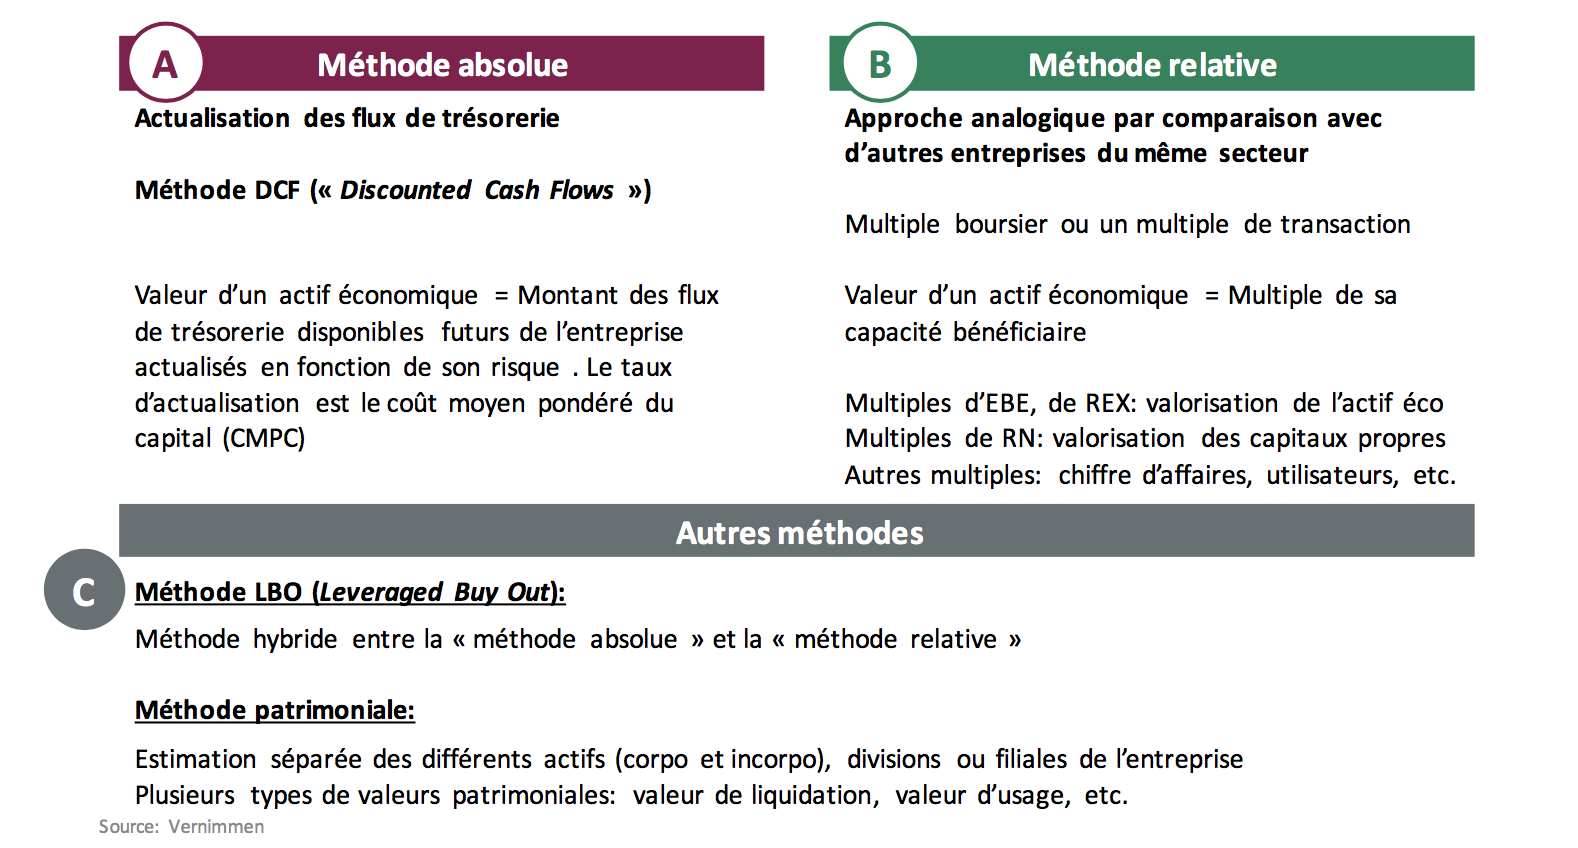
\includegraphics[scale=0.5]{img/im2}
	\label{fig:1}
\end{figure}

\subsection{Méthode absolue} % (fold)
\label{sub:méthode_absolue}

On a :
\[
	VE= \sum_{i=1} \frac{FCF_i}{(1+WACC)^i} + \frac{VT}{(1+WACC)^n}
\]

Il nous faut donc calculer 2 éléments :

\begin{itemize}[label=\ding{69}]

	\item Free Cash Flow : 
	\[
		FCF=EBE-Impôt_{EBIT}\cdot EBIT - CAPEX +/- \Delta BFR
	\]
	Avec CAPEX étant les dépendese d'investissement.

	\item Valeur terminale (VT):
	On a dans ce cas 3 méthodes pour l'obtenir.

	\begin{figure}[H]
		\centering
		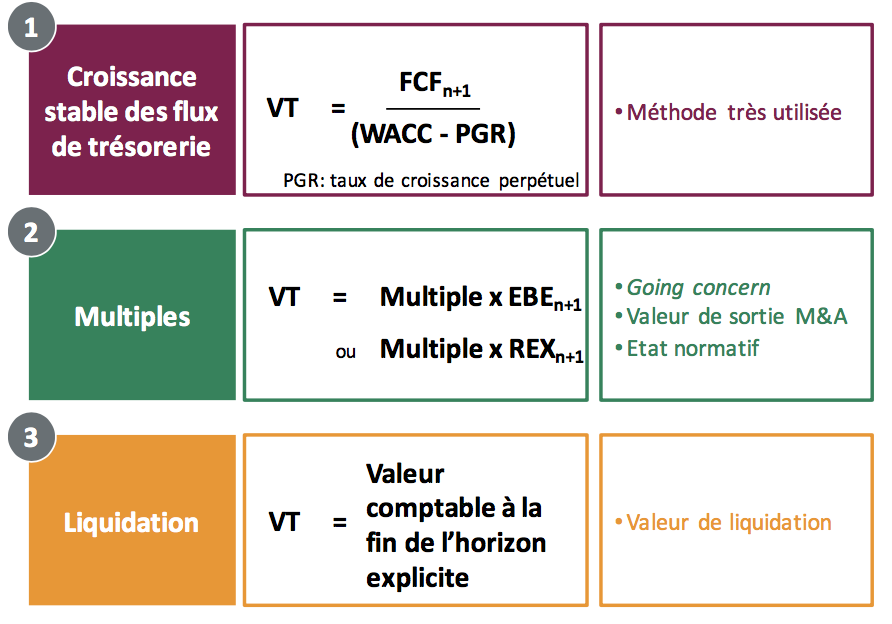
\includegraphics[scale=0.5]{img/im3}
	\end{figure}

\end{itemize}

Une autre élément essentiel est le WACC, ou CMPC. En d'autres mots le coût du capital. On a : 
\[
	CMPC=K_e\cdot \frac{CP}{CP+DFi} + K_F\cdot(1-IS) \cdot\frac{DFi}{CP+DFi}
\]
Avec $K_e$ le taux de rendement éxigé par les actionnaires, et $K_F$ le taux d'intérêt de chaque type d'emprunt.



% subsection méthode_absolue (end)

\subsection{Méthode relative} % (fold)
\label{sub:méthode_relative}

Il s'agit la de se comparer à d'autres entreprises du secteur. Plusieurs méthodes peuvent être utilisées on présente ici la méthode des ``Multiples Boursiers'', l'idée centrale restant la même pour toutes les méthodes.

 On vas donc analyser pour une série d'entreprises du marché les multiplicateurs $K_1^j$ et $K_2^j$ tels que $EBE^j=K_1^j$ et $RN^j=K_2^j$. Puis on peut determiner un intervalle de valeurs des fonds propres et du résultat net : 
\[
	I_{VE}=[\min K_1 \cdot EBE, \max K_1\cdot EBE] \quad I_{FP}=[\min K_2 \cdot EBE, \max K_2\cdot EBE]
\]
\emph{Note : Pour obtenir les FP à partir de VE  il faut soustraire la dette financière nette.}
% subsection méthode_relative (end)

\subsection{Méthode LBO} % (fold)
\label{sub:méthode_lbo}

Il s'agit l'á de calculer le TRI d'une LBO puis se poser la question que qu'elle valeur initiale nous aurait ammené à un tel TRI.

En sachant que TRI ($j$) est la valeur qui annule la VAN avec : 
\[
	VAN = -C+\sum_{j=1}^n\frac{CashFlow_j}{(1+WACC)^j}
\]

% subsection méthode (end)

% section la_valorisation (end)

\end{document}